\section{数据获取和图生成模型}

% 3 页

\subsection{数据来源}

先前的章节总结了常见的路由数据集在多样性和尺度上存在不适用于图网络的问题,因此本文将使用来自互联网和 DN42 两种分布式网路的数据。

其中互联网的路由数据来源于 RIPE RIS 的公开数据集\citing{ripe2021routing},它将经过更多的处理步骤以解决数据规模和冗余数据等问题。而 DN42 则是一个去中心化的的实验性社区网络,它的数据集来源于 DN42 全球路由收集器(Global Route Collector)的数据\citing{dn42us}。与 RIPE RIS 相似地,DN42 GRC \citing{dn422022mrt}也提供了 DN42 下几乎全部的路由信息。 

不同的是,由于 DN42 相对于管理规则更为严格的互联网而言具有更加扁平的结构\citing{dn42us},因而具有更强的分布式特点,同时由于其实验性的定位,会更频繁地发生 BGP 路由的异常,甚至能够合规地在一定范围内制造这样的异常以供研究用途,\citing{tsai2022design} 因此本文在互联网之外还使用了这一数据集,在后续的研究中也会借助 DN42 作为一些算法的案例分析。

如表格 \ref{dataset-compare} 所示,本研究采集了相近时间的来自两种网络的数据,并总结了以上两种数据来源的不同之处,可见它们在数据规模、复杂度和结构特点上都有所不同,本研究尝试通过两类截然不同的网络结构的数据集来研究模型在面对不同结构的网络路由上,是否能保持一致的准确度,以便测试模型的泛用性。

\begin{table}
    \caption{两种数据集的参数对比}
    \begin{tabular}{p{0.2\linewidth}p{0.3\linewidth}p{0.3\linewidth}}
        \toprule
                       & \textbf{RIPE RIS}                                & \textbf{DN42 GRC}              \\
        \midrule
        宣告的IP前缀 \newline(IPv4) & $\sim$1,000,000                                  & $\sim$800                      \\
        宣告的IP前缀 \newline(IPv6) & $\sim$170,000                                    & $\sim$700                      \\
        可观测到的自治系统      & $\sim$70,000                                     & $\sim$500                      \\
        更新频率           & 8 小时 (全量),                     \newline5 分钟 (增量) & 10 分钟 (1周内), \newline1 天 (一周外) \\
        网络关系与拓扑        & 对等+非对等                                           & (几乎完全)双向非对等                    \\
        \midrule
        本文使用           & 性能评估                                             & 对照分析                           \\
        \bottomrule
    \end{tabular}
    \label{dataset-compare}
\end{table}

路由收集器提供的数据大多使用 MRT 格式,它能够完整地记录路由表中的多种路由信息,在本章节的研究中,MRT 文件中的路由将在数据的预处理阶段被导出,其中的自治系统路径和社区属性等信息是以图\ref{c3_data-struct}中的形式被保存在层次性的数据结构中,以便于后续将拓扑信息和其它属性分离开来。

\begin{figure}[h]
    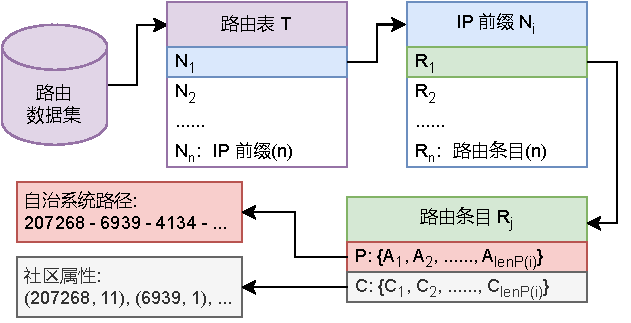
\includegraphics[width=0.7\linewidth]{chapter/c3_images/c3_data-struct.pdf}
    \caption{图网络路由数据集的组成结构,依层次为:路由数据集、路由表、网络前缀、路由及其包含的路径和社区属性}
    \label{c3_data-struct}
\end{figure}

\subsection{基于自治系统逻辑拓扑关系的图网络数据构建}

\subsubsection{层次结构分析}

\begin{figure}[h]
    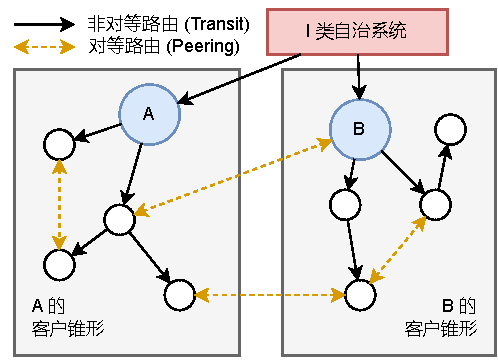
\includegraphics[width=0.6\linewidth]{chapter/c3_images/c3_dataset-layers.pdf}
    \caption{路由数据集的层次分解。由 A 和 B 建立的两个客户锥形之间存在的对等路由}
    \label{c3_dataset-layers}
\end{figure}

图 \ref{c3_as-distance} 的结果能够反映出,广域网络的一些连边事实上并不在路由信息的传递中扮演作用,这导致了完全通过网络路由数据集构建的图网络与真实路由系统的运作模式不一致,例如图中的平均自治系统长度的差异,而这些差异最终都将体现在模型的运行效果上。因而,为了实现下游模型训练效果的优化,需要从广域网络路由协议的角度去分析这些在路由过程中不扮演消息传递角色的路由,并将其从构造的图中去除。

通过对广域网路由模型的分析,广域网络的路由可以被抽象为一个类树状结构加上一些随机噪声连边,这种现象能够通过自治系统的互联模式很好的解释。如图 \ref{c3_dataset-layers} 所示,由于互联网络是由非对等互联路由和对等互联路由共同构成,前者具有一定的层次性,因而形成一种类树状结构;而后者则存在一定的无序性,因此能够随机地连接网络中的节点。由于对等路由仅仅在直接连接的自治系统之间交换路由,并不会传递其它自治系统的路由,因此这部分的路由在用于异常检测上时能够被移除而不影响异常检测的效果。

为了验证上述猜想,首先在图上定义对等路由:

对于一个路由表${R_i}$,某两个节点 $V_a$ 和 $V_b$ 的之间的路由$R_p$是自治系统长度为 1 的路由,假设其连边为 $E_p$,则它是对等(Peering)路由,当且仅当路由表${R_i}$的任意路由 $R_k$ 中不包含长度大于1,且路径末端为连边 $E_p$ 的自治系统路径。或者以公式\ref{peering_route}的方式表示:
\begin{equation} \label{peering_route}
R_p = \{P: \{E_p<V_a, V_b>\} \}, 
\forall R_k \in \{R_i\} \parallel len(P_k) \geq 1, E_p \neq last(P_k \in R_k)
\end{equation}

随后,为了研究现有数据集中的路由类型的分布状况,本研究使用了 RIPE RIS 和 DN42 在 2022年12月的数据集,对数据内节点介数中心度与它们的对等/非对等(Peering/Transit)路由的数量做出了统计和对比。实验结果如图 \ref{c3_route-centrality} 所示,可以从图中发现,互联网的非对等路由更具结构性,越具有中心度的节点,将具有越高的非对等路由,而对等路由则在大部分节点上呈现出随机的分布;作为对照,DN42 这类分布式网络由于大部分节点间完全通过双向非对等路由的形式进行路由交换,在路由数量与其介数中心度的关联上并没有互联网数据集密切。

\begin{figure}[h]
    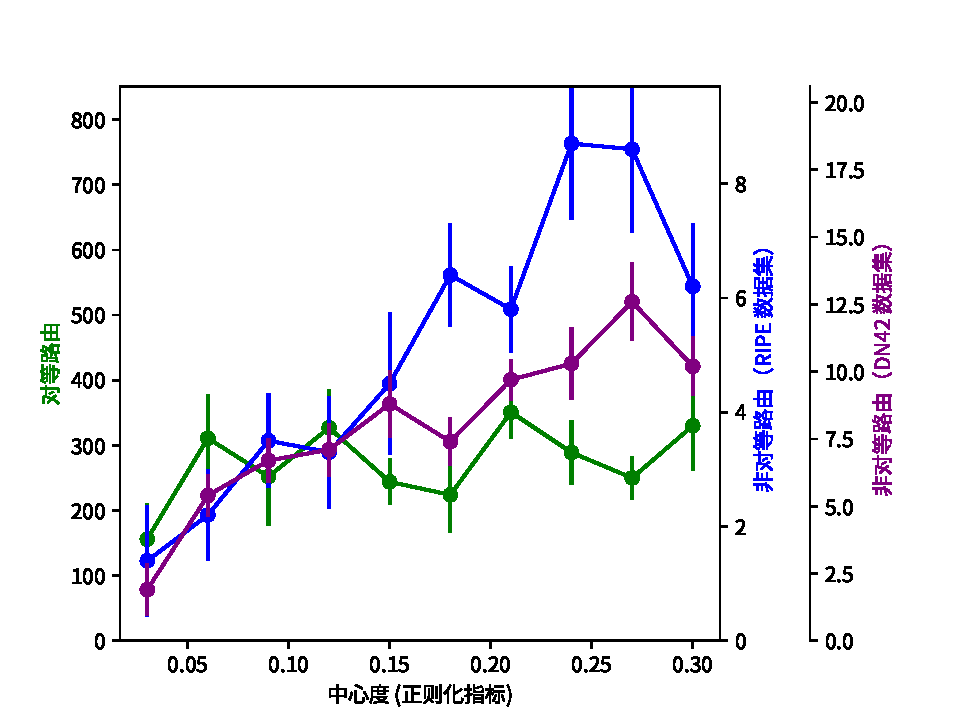
\includegraphics[width=0.9\linewidth]{chapter/c3_images/c3_route-centrality.pdf}
    \caption{路由数据集上对等/非对等(Peering/Transit)路由的数量与中心度的关联}
    \label{c3_route-centrality}
\end{figure}

假如去除路由系统中的对等连边,是否会有度为0的孤立节点产生是另一个因此出现的问题。根据路由条目沿非对等路由传播的定义,某个节点 $V_a$ 与 网络中任一节点互通,且并非通过对等方式互通(即 $d(V_a)\neq n-1$),则$V_a$与任一I类自治系统应当存在非对等路由关系,而根据I类自治系统的定义,没有任何节点向它们提供非对等路由,因此它必然存在一条通往I类自治系统的非对等路由。通过以上方式,能够证明,所有能够访问全部广域网的节点,要么与其余全部节点存在对等路由,要么存在至少一条可进入数据集的非对等路由。

% 对于自治系统节点 $V_a$,而言,设子图区域 $G_z = <\{V - V_a, E - E_a\}>$,其中 $E_a = \{ \forall E_k(V_{from}, V_{to}) \in E, if (V_{from} = V_a \parallel V_{to} = V_a ) \}$。假设 $V_a$ 不存在 Transit 路由,对于 $V_a$ 的临接节点集 $V_{nei}$,一定存在 $V_{nei} \leftrightarrow V_a $,即路由双向可达,由于 Peering 路由长度一定为 1,则对于 $V_a$ 的非临接节点集 $V - V_{nei}$ 一定在 $G_z$ 上存在一条通向 $V_a$ 的 Transit 路由,为了保证 $V_a$ 一定在 $V_{sample} \in V - V_a \in G_z$ 为起点的采样数据集中出现,即 $E\{P(V_a \rightarrow V_{sample})\} = 1$,要么 $V_{nei} =V - V_a$,要么 $V_a$ 存在至少一条 Transit 路由。

事实上,上述区域 $G_z$ 被称为DFZ(Default-Free Zone)区域,其被定义为拥有全部广域网路由的自治系统路由器集合。即使对等路由在实际网络中存在流量交换的意义,在此场景下仍然能够将其去除从而不影响图网络整体在异常检测上表现出的结构性。

\subsubsection{图生成算法}

在验证了上述假设的条件下,对路由数据的处理问题转化为了如何在现有的数据中提取并去除对等路由。

在此基础上,路由数据集的图生成算法定义如表 \ref{algo-datagen-topo} 所示。该算法能够通过上述方法去除没有对异常检测存在意义的对等互联路径,从而输出一张更具结构性特征的广域网路由拓扑图,从而达到降低网络复杂度、稠密度的效果。

\begin{algorithm}[H]
    \KwData{输入路由集合 \{$R_i$\} 和预先定义的I类ISP 表 $V_{t1}$}
    \KwResult{输出一份由此数据生成的数据集}
    初始化图网络:
    $G<V=\{\},E=\{\}>$\;
    提取路由路径:
    $\{P_i \in R_i\}$\;
    初始图网络生成:
    \For{$\{V_a, E_{ab}, V_b\} \in P_i$}{
    $G<V+=\{V_a, V_b\},E+={E_{ab}}>$
    }
    \For{每个非I类自治系统的节点$V_i \notin V_{t1}$,检查它们的连接 $e_i$:}{
        \If{$e_i$ 满足对等路由的条件}{
            从图中删除它: $G<V, E=E-e_i>$
        }
    }
    输出网络 $G$\;
    \caption{基于逻辑拓扑关系的路由图网络生成算法}
    \label{algo-datagen-topo}
\end{algorithm}

\subsection{基于自治系统路由相似度度量的图网络数据构建}

除了直接使用数据集中的路由数据进行图的拓扑构建外,还能使用原数据的节点相似度度量对图进行构建。这是对于过于冗余的原数据集的另一种利用方法,该方法将其转换为节点间路由度量的带权图,这能够将原本的路由拓扑图变得稀疏化,同时将冗余数据转化为正则化的指标。

虽然介数中心度在反映路由中心度上更具优势,但它的计算复杂度在面对互联网数据集的规模(>5000万条连边)的情况下过高,而在图网络中,基于余弦相似度的节点表征方法相比而言更加实际,它通过采样节点的邻居信息并实现对节点之间的相似度度量,并更加快速,适合使用在数据集的处理上。它的定义如公式 \ref{cos_dist} 所示。
\begin{equation} \label{cos_dist}
d_{cos}(V_A,V_B) = \frac{\Sigma_{nei} V_i^A V_i^B}{\sqrt{\Sigma_{nei} (V_i^A)^2} \sqrt{\Sigma_{nei} (V_i^B)^2}}
\end{equation}
% 公式

根据上述定义,使用以下算法利用相似度度量对原始数据集进行处理:

% 构图算法表格

\begin{algorithm}[H]
    \KwData{输入路由集合 $\{R_i\}$}
    \KwResult{输出一份由此数据生成的数据集}
    初始化图网络:
    $G<V=\{\},E=\{\}>$\;
    \For{每条路径 $\{P_i \in R_i\}$}{
        \For{路径上的相邻两个自治系统 $(V_a, V_b) \in P_i$}{
            对边赋权重:$e(V_a, V_b) += d_{cos}(V_a, V_b)$
        }
    }
    \For{图 $G$ 中的每个顶点 $\{V_i \in V \in G\}$}{
        \For{顶点上的每条边 $(V_a, V_b) \in E(V_i)$}{
            \eIf{进行 top-k 计算:$topk(E(V_a, V_b))$}{
                保留边 $E(V_a, V_b)$ \;
            }
            {
                删除边 $E(V_a, V_b)$ \;
            }
        }
    }
    输出网络 $G$\;
    \caption{基于路由相似度度量的路由图网络生成算法}
    \label{algo-datagen-sim}
\end{algorithm}

如表 \ref{algo-datagen-sim} 所示的算法描述,在获取数据集后,对路径上每一对自治系统节点间的相似度进行余弦相似度计算,将其作为邻接矩阵的权值。对于生成的临接矩阵,它是一个全连接的完全图,使用每节点 topk 权值的平均值作为分界值,从而将其变为更加稀疏的图网络。